% -*- TeX-master: "../dipole_ilya_paper.tex" -*-
\section{Fabrication}
\red{Thickness of aluminium size of chip }

\red{Glued to  a pcb and bonded  with gold wires,  connectio input and output  to coax
lines.}

\begin{figure}[h]
  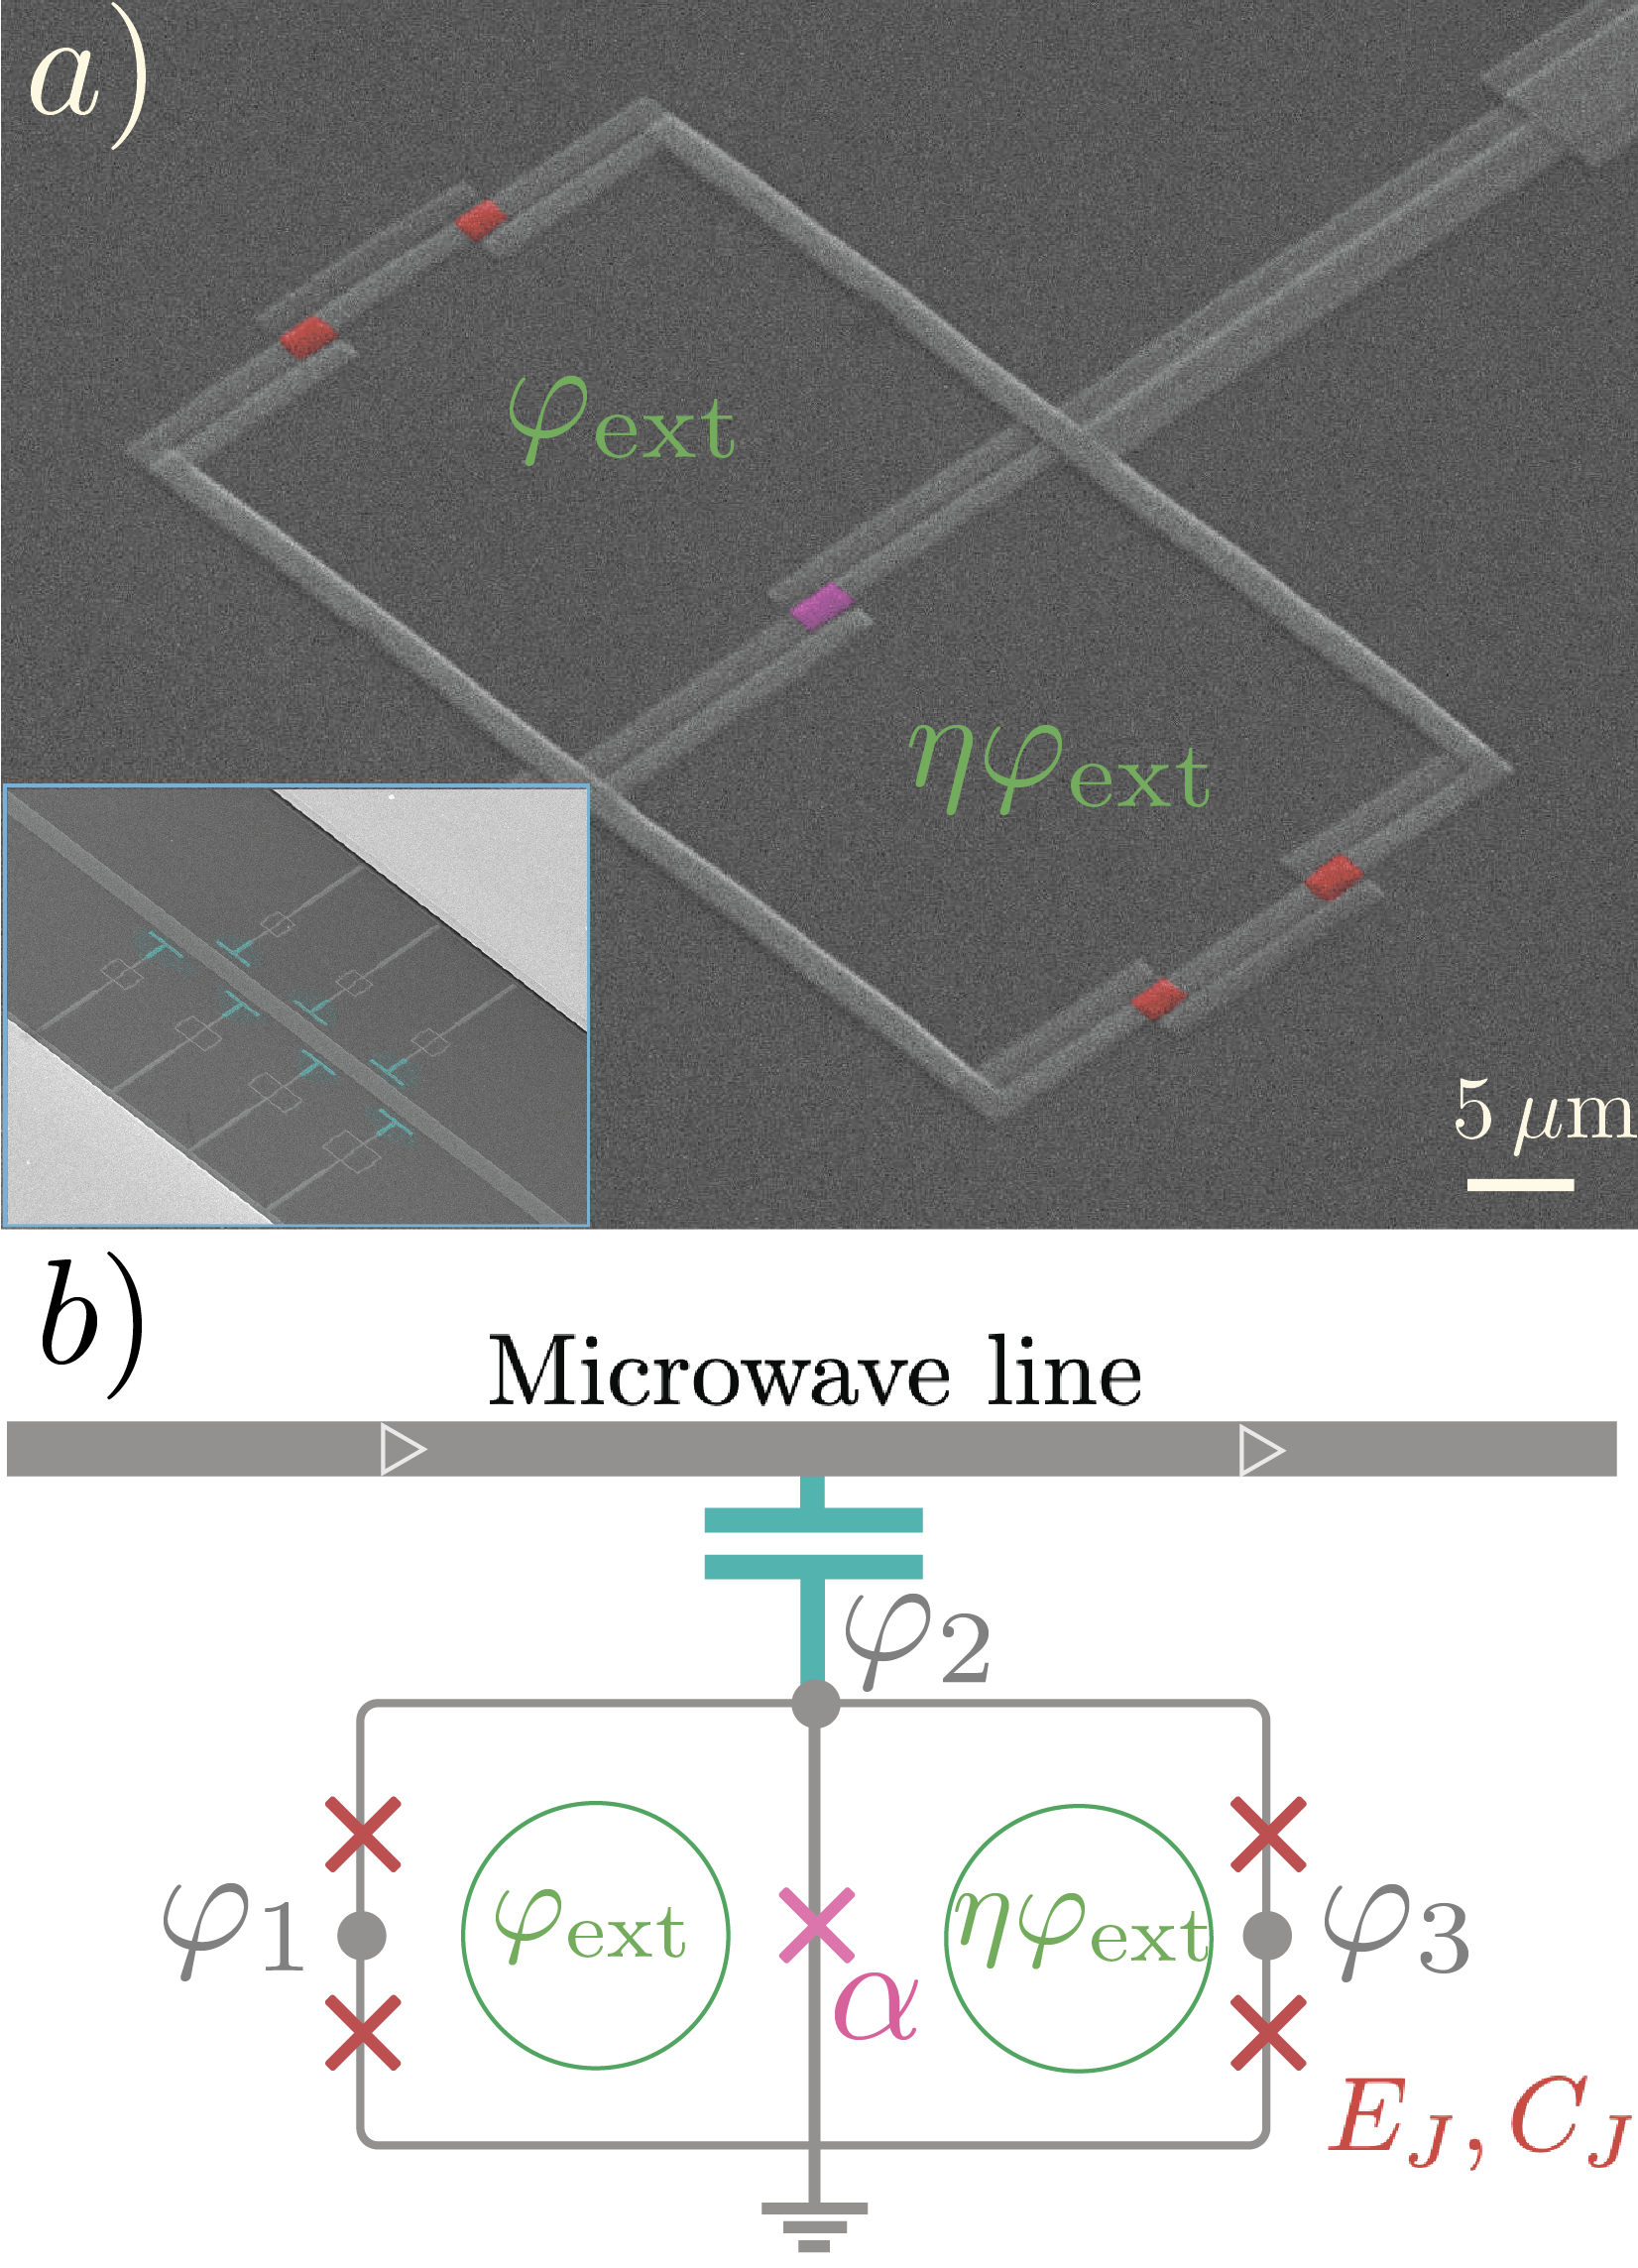
\includegraphics[height=10.5cm]{figure1_v3}
  \caption{\small Geometry of a twin qubit: a) Scanning electron microscope image
    of  the  qubit flux  with  phase  biases  $ \varphi  $,  $  \eta\varphi  $ applied  to  it's
    superconducting loops. The repeated line  structures are the byproduct of the
    double-angle  evaporation  of aluminum  that  creates  the Al-AlO$_x$-Al  JJs
    highlighted in red and pink. The qubit  is coupled to the microwave line with
    a T-shaped capacitor (inset); b) The  twin qubit is a symmetrical arrangement
    of  two individual  flux  qubits.  The  central junction  has  an energy  and
    capacitance  of  $ \alpha  E_{J}$,  $\alpha  C$ compared  with  the  outside values  of
    E$_J$C$_J$.}
  \label{fig:setup}
\end{figure}

%% Describe fabrication
\noindent The qubit  is fabricated on the undoped silicon  substrate.  A coplanar
transmission line with impedance  $ Z_{0} \sim 50\,\Omega $ is run  to an opening between
the ground planes in the center of the chip, see Fig~\ref{fig:setup}. Twin qubits
and T-shaped capacitors  coupling qubits to the transmission  line are fabricated
simultaneously   using    the   shadow   evaporation   technique    of   aluminum
\cite{wu2013}. These  steps result in  a 5-JJ structure  of Fig.~\ref{fig:setup},
each JJ with 2 squares and  an area of \iunit{200\times200}{nm$^2$}.  Measurements are
performed in  a 14\,mK  environment of  a dilution  refrigerator so  that thermal
activation of  GHz frequency transitions  are suppressed.  All  microwave signals
probing the system pass through a  single transmission line equipped with
a standard set  of attenuators on the  input side, and circulators  and low noise
amplifiers on  the output  side.  This facilitates  power conversion  between the
laboratory equipment and qubit microwaves.

Our pilot experiment did  not to go to the depths of  using chemical and physical
treatment of  the substrate  surface to  remove two-level  system defects  in the
silicon  oxide layer  \cite{earnest2018}  or employing  multi-stage shielding  to
eliminate  stray infrared  light  during  measurement \cite{barends2011}. We plan on doing these improvements in further development cycles  of the twin qubit.




%% Explain how other new  qubits have been fabricated with grooves  and HF - this
%% is down the line for this type of geometry

%%% Local Variables:
%%% mode: latex
%%% TeX-master: "../dipole_ilya_paper"
%%% End:
